% !TEX root = ../../main.tex

% --------------------------------------
% labels: \label{mil4:res:[type]:[name]}
% --------------------------------------
% PAST TENSE


As functions of wavenumber $k$, we plot the transfer function for a set of angular wavenumbers $\ell \in \{\, 6,\, 100,\, 200,\, 500,\, 1000 \,\}$ in~\cref{mil4:res:fig:transfer}. For the a smaller range of values of $k$, we also plot the interesting part of the integrand in the expression for the CMB power spectrum. 
\begin{figure}[!ht]
    \centering
    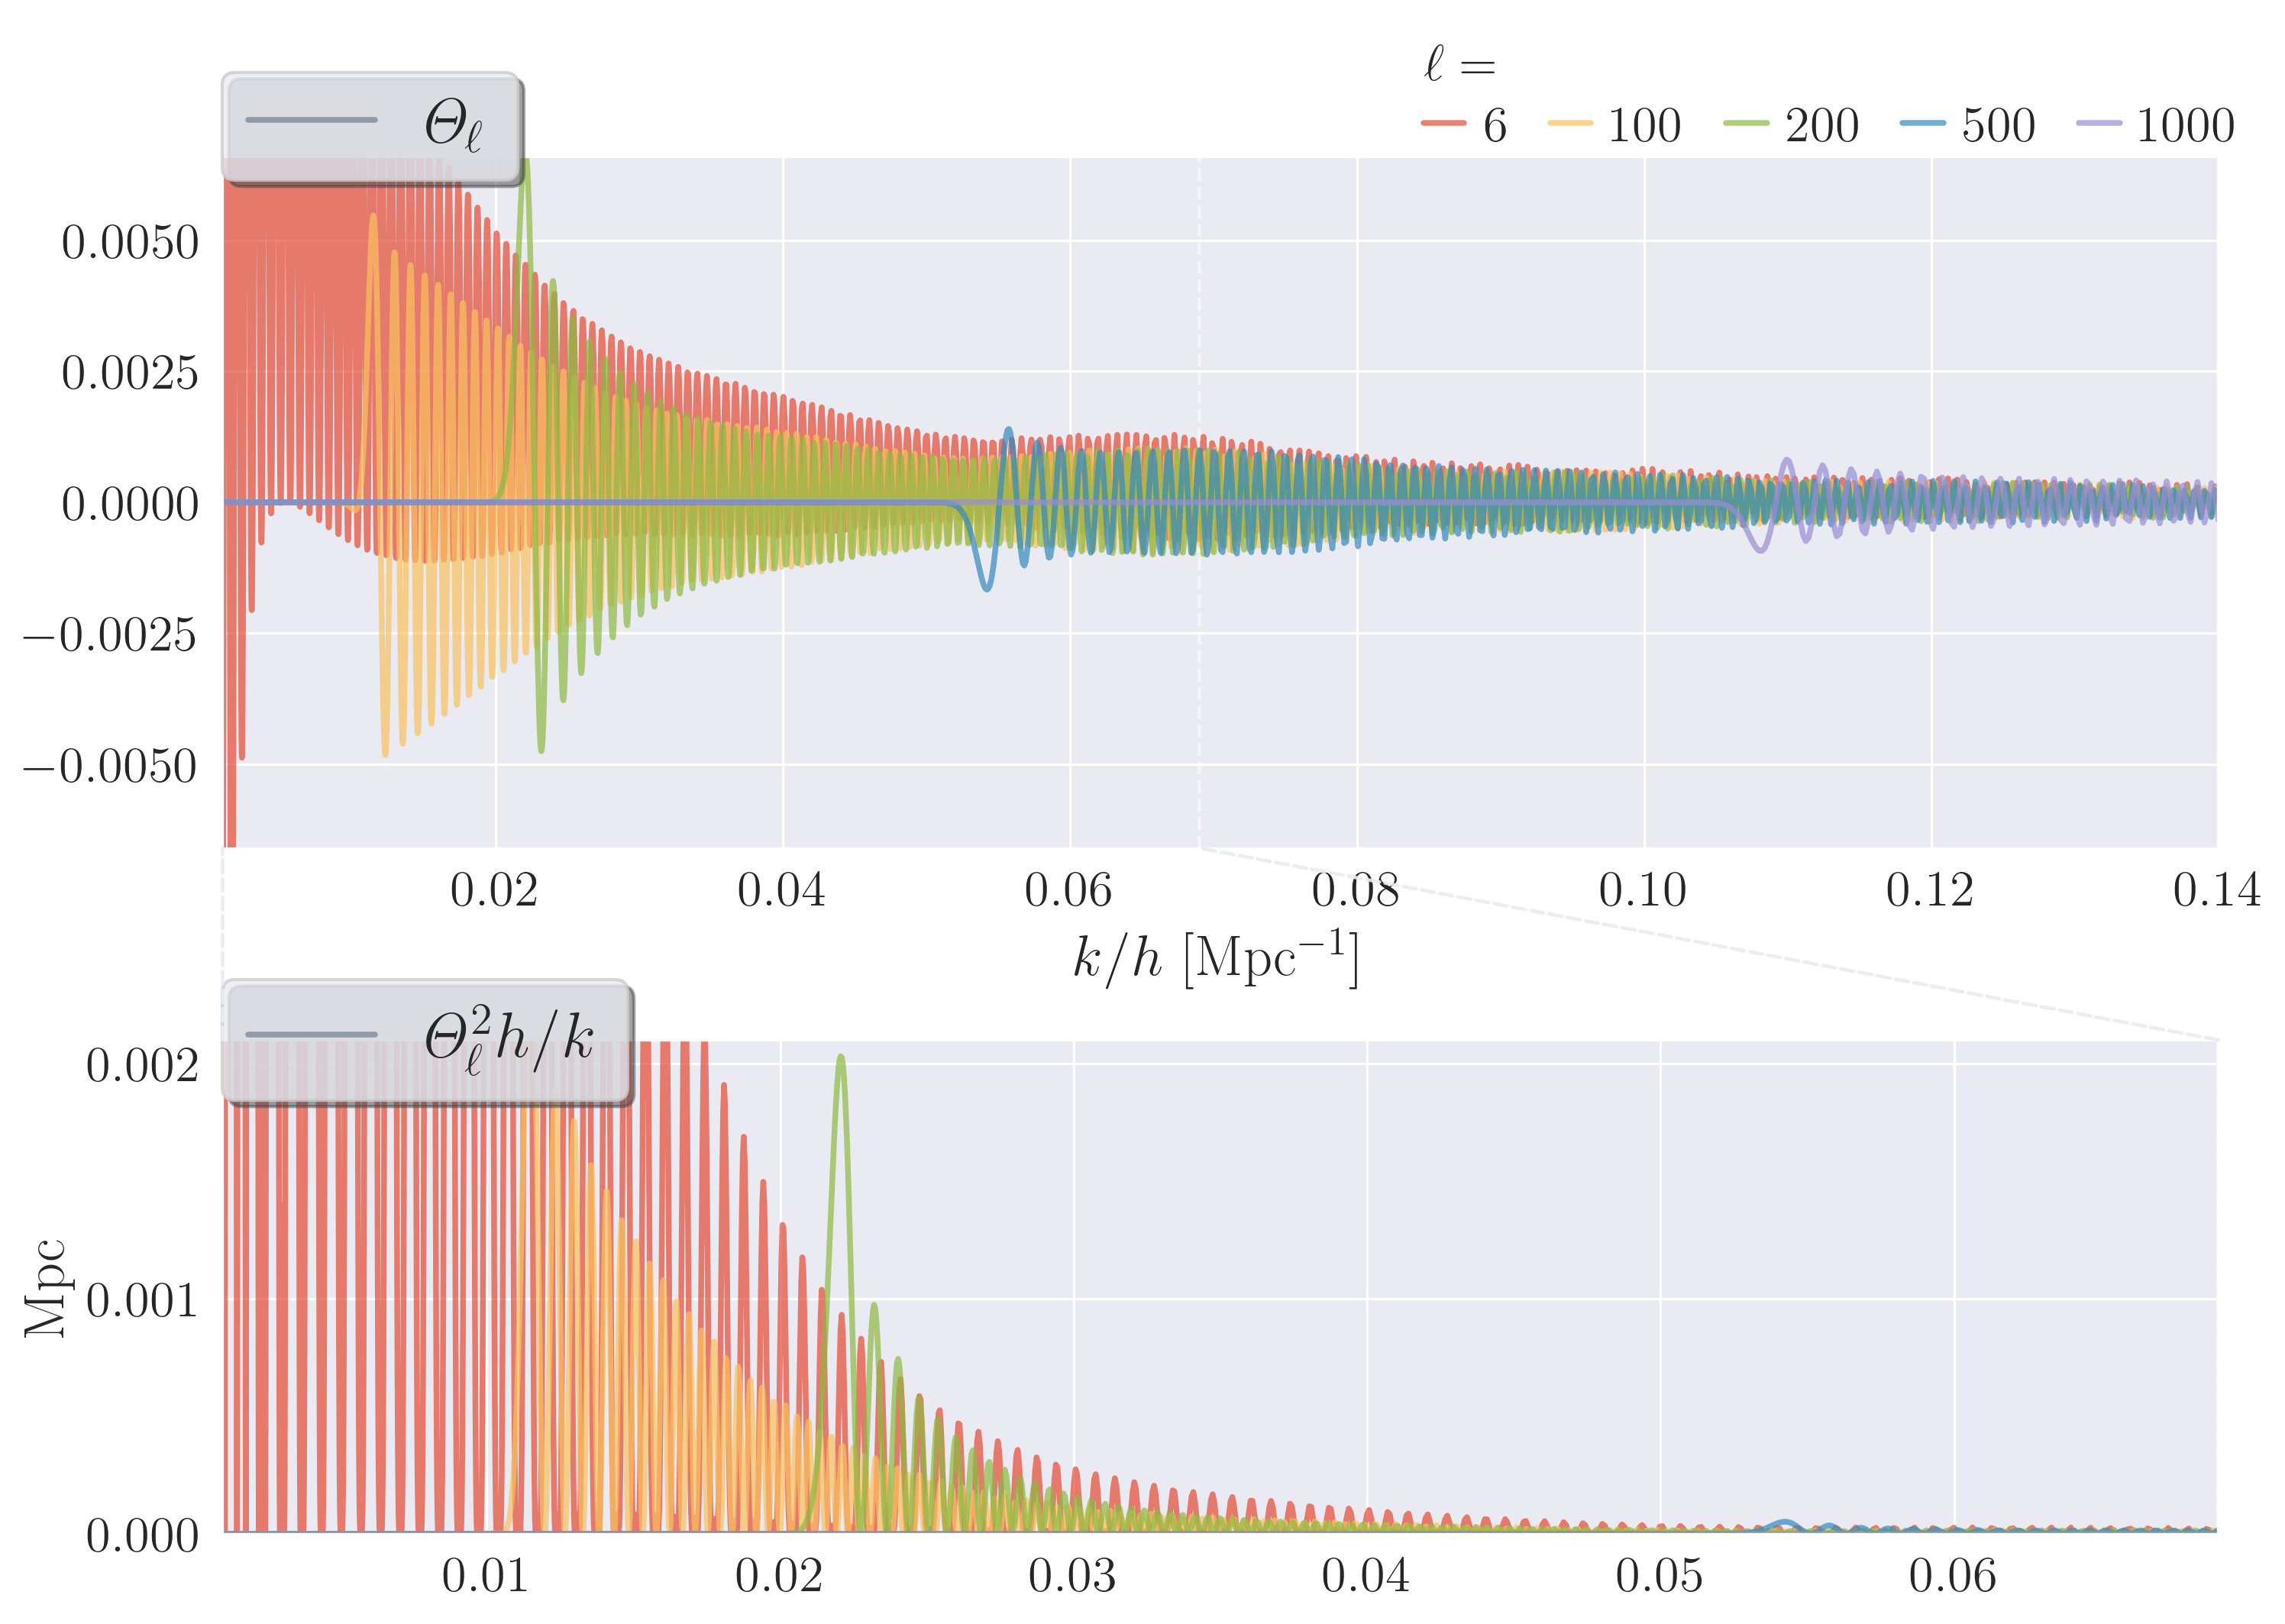
\includegraphics[width=\linewidth]{milestone4/Theta_ell.png} 
    \caption{The photon transfer functions $\Theta_\ell(0, k)$ as functions of wavenumber $k$ for a set of angular wavenumbers $\ell$. We extracted a part of the $x$-axis for which to show $\ell(\ell+1)\cross \frac{1}{k}\abs{\Theta_\ell(0,k)}^2$ as functions of $k$, now with emphasis on the fundamental scale for which $k_n = nk_1$.}
    %Upper panel: Plainly $\Theta_\ell(0, k)$. Lower panel: For a part of the  $\frac{\Theta^2_\ell(0,k)}{k}$.} 
\label[fig]{mil4:res:fig:transfer}
\end{figure}

The CMB power spectrum is presented in~\cref{mil4:res:fig:CMB_power}. Note that we used the scaled quantity $\mathcal{D}(\ell)$. The different contributions to the CMB anisotropy were overplotted, as well as the cosmic variance from~\cref{mil4:theo:eq:cosmic_variance}. We included observational data from~\citet{Planckdata} for low $\ell$. Observational data become less relevant for $\ell \ga 200$ as effects of e.g.\ neutrinos are non-negligible at these scales.
\begin{figure}[!ht]
    \centering
    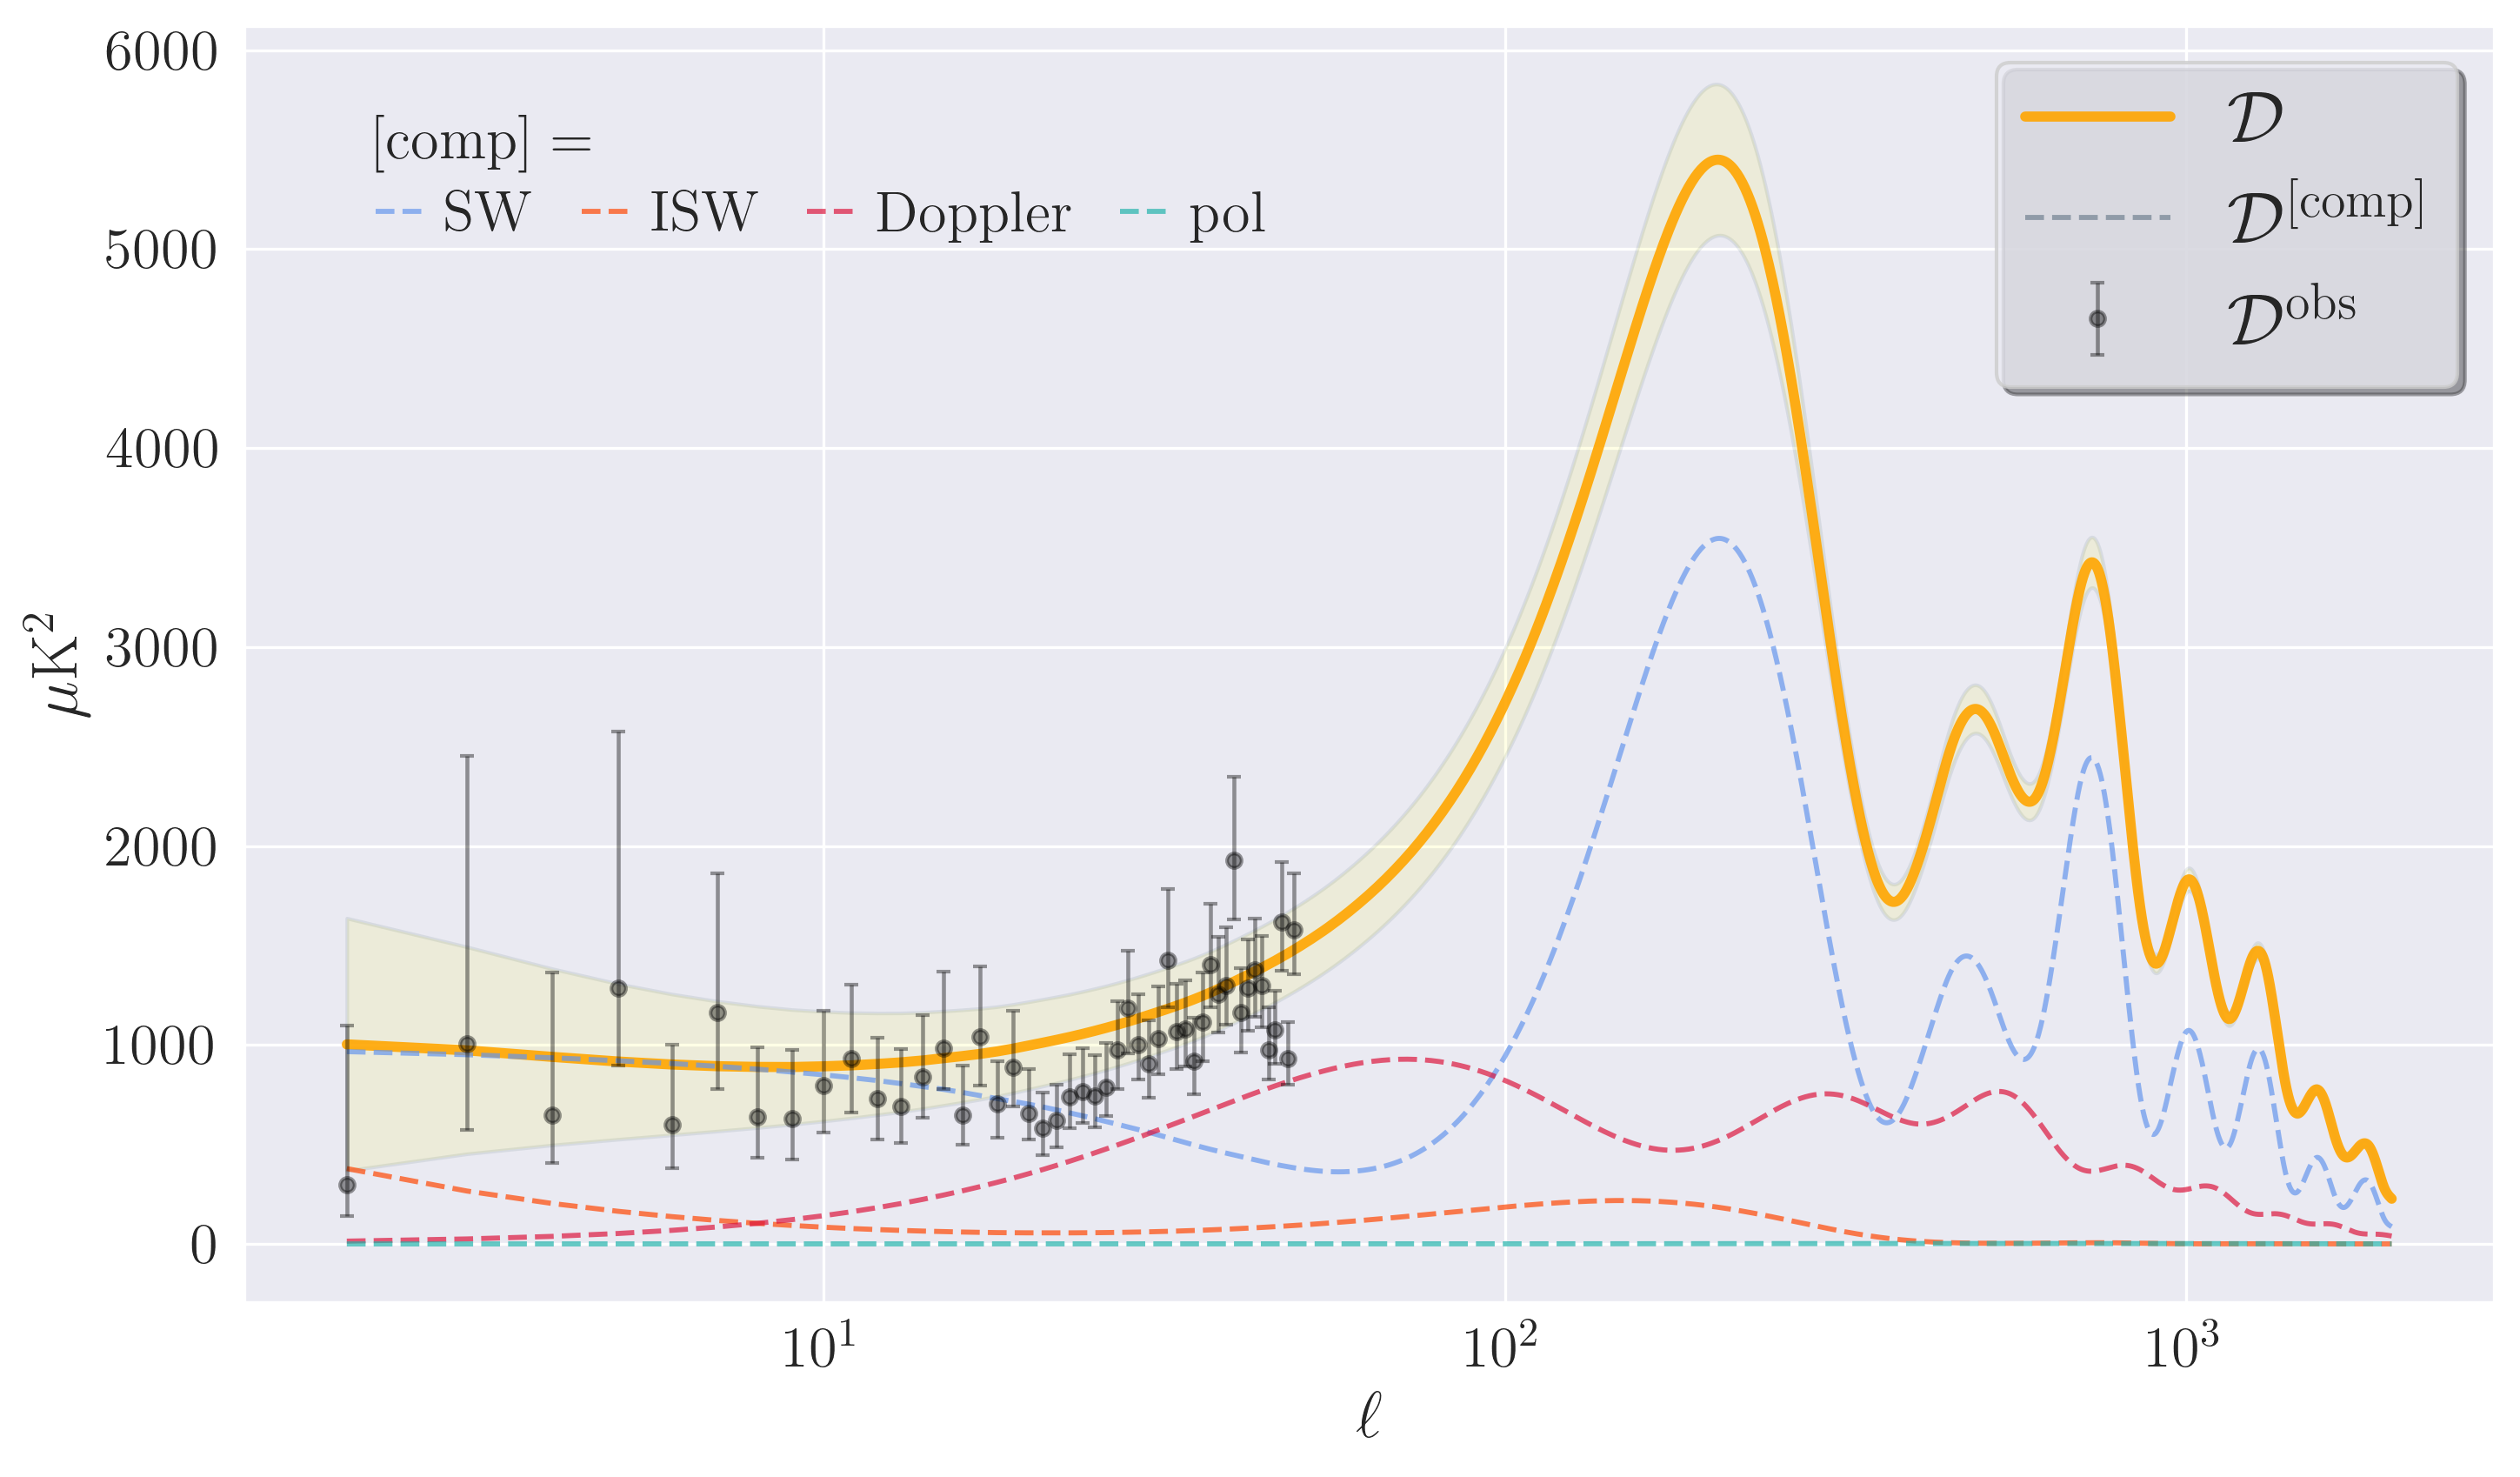
\includegraphics[width=\linewidth]{milestone4/CMB_power_spectrum.png} 
    \caption{The scaled CMB power spectrum $\mathcal{D}(\ell)$ as function of multipole moment $\ell$. The shaded region represents the fundamental cosmic variance. Upper axis demonstrates corresponding angular scale $\sim 180\degr /\ell$. Observational data are included for large scales.} 
\label[fig]{mil4:res:fig:CMB_power}
\end{figure}
The contributions to the CMB spectrum were calculated as follows, where $\mathrm{[comp]}\in \{\,\mathrm{SW},\,\mathrm{ISW},\,\mathrm{Doppler},\,\mathrm{pol} \,\}$ are the terms in the source function ($\St(x,k) \supset (\mathrm{[comp]})$, see~\cref{mil4:theo:eq:source_function_four_terms}) given by~\cref{mil4:theo:eq:source_terms}:
\begin{equation}
\begin{split}
    &\mathcal{D}(\ell)^\mathrm{[comp]} = \frac{\ell (\ell +1 ) \TCMB^2}{2\pi} C(\ell)^\mathrm{[comp]}\,; \\
    &\quad C(\ell)^\mathrm{[comp]} =  4\pi \int_0^{\infty} \dx{k} \frac{\abs{\Theta_\ell^{\mathrm{[comp]}}(0,k)}^2}{k} \Delta_\mathcal{R}^2(k)\,; \\
    &\quad\quad \Theta_\ell^\mathrm{[comp]}(0,k) = \int_{-\infty}^0 \dx{x}(\mathrm{[comp]}) j_\ell(k\left[\eta_0 -\eta(x)\right] )
\end{split}
\end{equation}

We found the fundametal tone at $\ell_1 = 205$. The next two peaks werw located at $\ell_2=490$ and $\ell_3 = 727$. Higher peaks were found at $\ell_4=1008$, $\ell_5=1273$, $\ell_6=1552$ and $\ell_7=1825$.

In figure~\cref{mil4:res:fig:matter_power} is plotted the total matter power spectrum. Observational data from~\citet{wmap_act} and~\citet{Planckdata} is shown in the same figure. Discrepancy is significantly larger for smaller scales.
\begin{figure}[!ht]
    \centering
    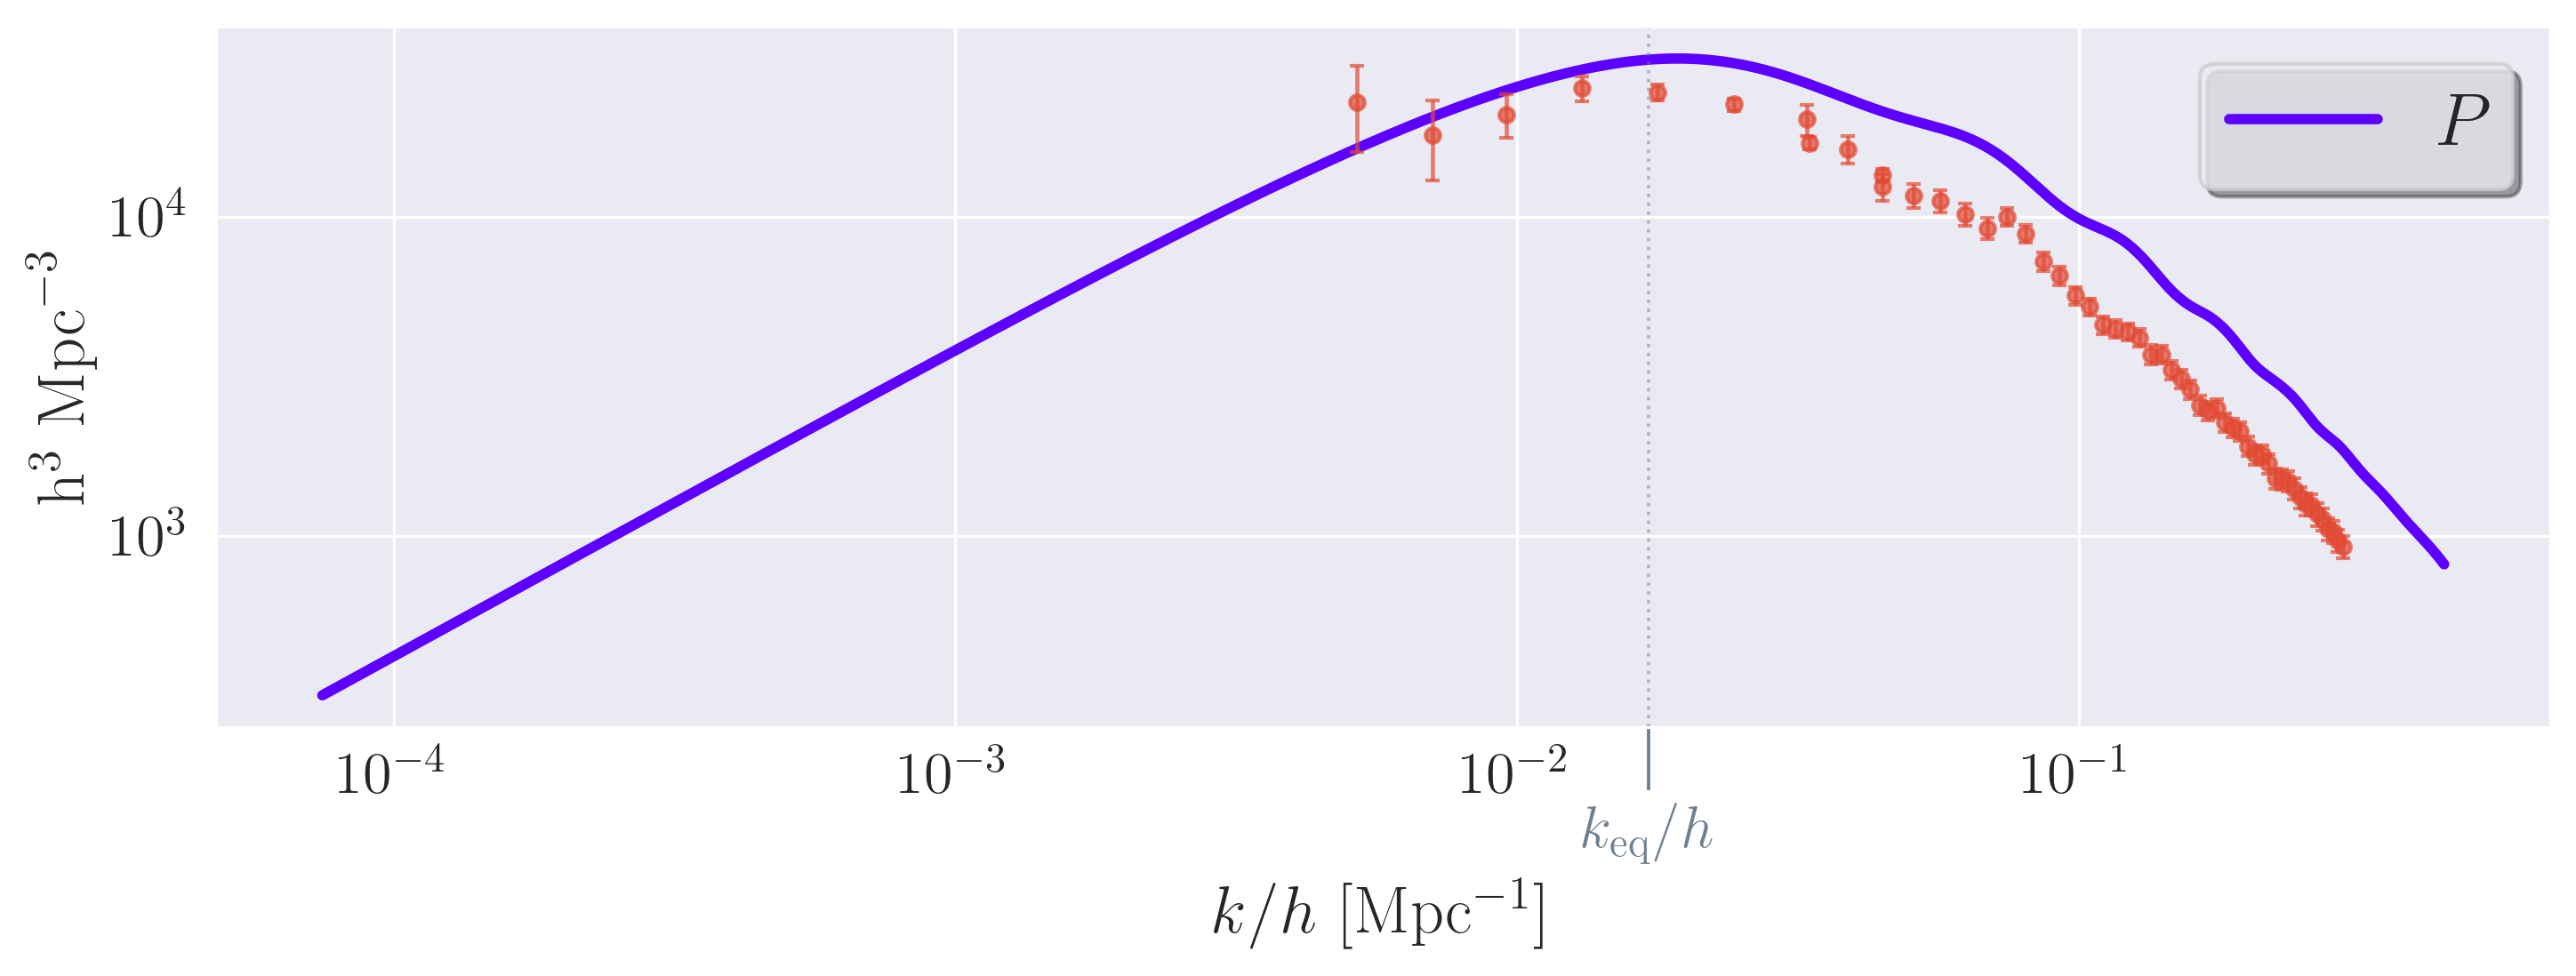
\includegraphics[width=\linewidth]{milestone4/matter_power_spectrum.png} 
    \caption{The total matter power spectrum (today) $P\ped{m0}(k)$ as function of wavenumber $k$. Both axes are logarithmic. The equality scale $k\ped{eq}$ is demonstrated by a vertical dotted line. The individual contributions from CDM and baryons and observational data are included.} 
\label[fig]{mil4:res:fig:matter_power}
\end{figure}
